E como trabalharam para juntar aquele feno! Mas o esforço foi recompensado, pois a colheita deu um
resultado muito melhor do que esperavam.

Por vezes, a tarefa foi dura, os implementos destinavam-se ao uso de seres humanos e foi uma enorme
desvantagem o fato de nenhum bicho poder utilizar ferramentas que exigissem a posição em pé sobre as
patas traseiras. Mas os porcos eram tão imaginosos que conseguiram contornar todas as dificuldades. Os
cavalos conheciam cada palmo do terreno e na realidade sabiam ceifar e raspar muito melhor do que
Jones e os empregados, Os porcos não trabalhavam,apromiadamente , mas dirigiam e supervisionavam o
trabalho dos outros. Donos de conhecimentos maiores, era natural que assumissem a liderança. Sansão e
Quitéria atrelavam-se à ceifadeira ou à grade (naturalmente não havia mais necessidade de freios e
rédeas) e andavam pelo campo para lá e para cá, com um porco atrás gritando "Eia, camarada!" ou "A
volta, agora, camarada!", conforme o caso. E cada animal, até os mais modestos, trabalhou para colher e
juntar o feno. Até os patos e as galinhas andavam o dia inteiro sob o sol, carregando no bico pequeninos
feixes de feno. Enfim, terminaram a colheita em dois dias antes do tempo que Jones e seus empregados
normalmente levavam. Mas, além disso, foi a maior colheita que jamais se realizara ali. Não houve
qualquer desperdício; as galinhas e os patos, com sua vista penetrante, juntaram até o menor talinho. E
nenhum animal na granja roubou sequer uma bocada.  

%Imagem
\begin{figure}[h]
	\vspace{-15mm}
	\centering % Centralizar
	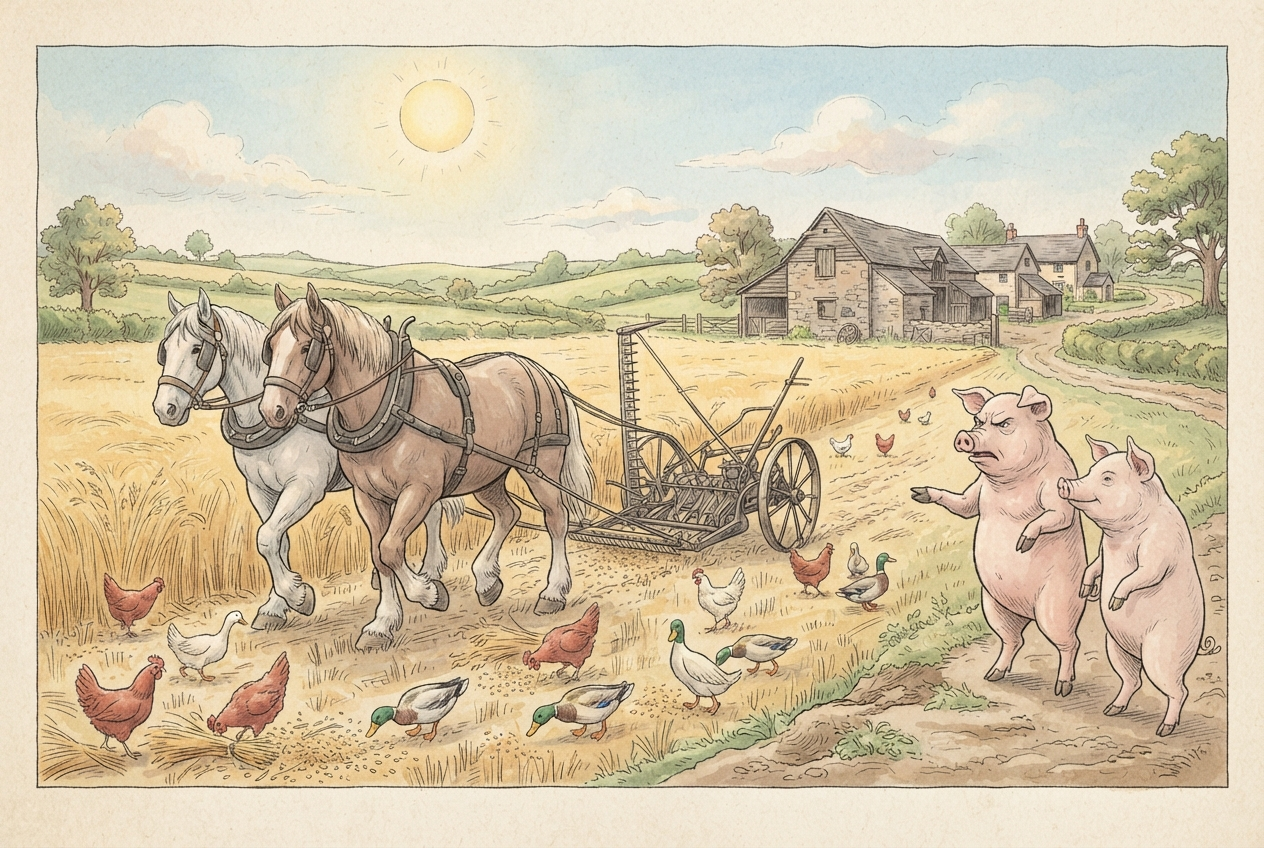
\includegraphics[scale=0.3]{img/imagemCap3} % arquivo da imagem.
	\caption{Coleita de feno.} % Legenda da imagem.
\end{figure}

Durante todo aquele verão o trabalho da granja andou como um relógio. Os bichos, felizes como nunca.
Cada bocado de comida constituía um extremo prazer, agora que a comida era realmente deles,
produzida por eles e para eles, em vez de distribuída em pequenas quantidades por um dono cheio de má
vontade. Ausentes os inúteis parasitas humanos, mais sobrava para cada um. Havia também mais lazer,
muito embora os animais fossem inexperientes nisso. Encontraram muitas dificuldades - por exemplo, no
fim do ano, quando colheram os cereais, foram obrigados a pisá-los, à moda antiga, e soprar as cascas,
pois a granja não possuía uma debulhadeira -, mas os porcos, com a inteligência, e Sansão, com seus
músculos fantásticos, sobrepujavam-nas. Sansão era a admiração de todos. Já era trabalhador no tempo
de Jones; agora, como que valia por três. Dias houve em que todo trabalho da granja parecia recair sobre
seus fortes ombros. Da manhã à noite lá estava ele, puxando e empurrando, sempre, no lugar onde o
trabalho era mais pesado. Fizera um trato com um dos galos para ser chamado meia hora mais cedo que
os demais, todas as manhãs, e empregava esse tempo em trabalho voluntário no que parecesse mais
necessário. Sua solução para cada problema, para cada contratempo, era "Trabalharei mais ainda", frase
que adotara como seu lema particular.

Cada qual trabalhava de acordo com sua capacidade. As galinhas e os patos, por exemplo, economizaram
cinco baldes de trigo, na colheita, juntando os grãos extraviados. Ninguém roubava, ninguém
resmungava a respeito das rações. A discórdia, as mordidas, o ciúme, coisas normais nos velhos tempos,
tinham quase desaparecido. Ninguém se esquivava ao trabalho - ou quase ninguém. Ë bem verdade que
Mimosa não gostava de levantar cedo e costumava abandonar o trabalho antes dos demais, sob o pretexto
de estar com uma pedra encravada no casco. E o comportamento do gato era um tanto estranho. Em
seguida notou-se que ele nunca podia ser encontrado quando havia trabalho por fazer. Desaparecia
durante várias horas consecutivas e voltava a aparecer à hora das refeições, ou à tardinha, após o fim dos
trabalhos, como se nada houvesse acontecido. Apresentava, porém, desculpas tão boas e rosnava de
maneira tão carinhosa, que era impossível não crer em suas boas intenções. O velho Benjamim, o burro,
nada mudara, após a Revolução. Executava sua tarefa da mesma forma obstinadamente lenta com que o
fazia nos tempos de Jones. Não se esquivava ao trabalho normal, mas nunca era voluntário para
extraordinários. Sobre a Revolução e seus resultados, não emitia opinião. Quando lhe perguntavam se
não era mais feliz, agora que Jones se havia ido, respondia apenas "Os burros vivem muito tempo.
Nenhum de vocês jamais viu um burro morto", e os outros tinham que contentar-se com essa obscura
resposta.

Aos domingos, não se trabalhava. A refeição da manhã era uma hora mais- tarde e, depois dela, havia
uma cerimônia que se realizava todas as semanas, indefectivelmente. Começava com o hasteamento da
bandeira. Bola-de-Neve achara, no depósito, uma velha toalha verde de mesa e pintara no centro, em
branco, um chifre e uma ferradura. Essa era bandeira que subia ao topo do mastro todos os domingos
pela manhã. O verde da bandeira, explicava Bola-de-Neve, representava os verdes campos da Inglaterra,
ao passo que o chifre e a ferradura simbolizavam a futura República dos Bichos, cujo advento teria lugar
no dia em que o gênero humano, enfim, desaparecesse. Após o hasteamento da bandeira, iam todos ao
grande celeiro, para assistir a uma assembléia geral conhecida como "a Reunião". Lá planejavam o
trabalho da semana seguinte e discutiam as resoluções. Estas eram sempre apresentadas pelos porcos. Os
outros animais aprenderam a votar, mas nunca conseguiram imaginar uma resolução por conta própria.
Bola-de-Neve e Napoleão eram sempre mais ativos nos debates. Notou-se, porém, que dois nunca
estavam de acordo: qualquer sugestão de um podia contar, na certa, com a oposição do outro.

Mesmo quando, se resolveu - coisa que, em si, não podia sofrer a objeção de ninguém - que o potreiro
situado além do pomar seria reservado para os animais aposentados, houve uma agitada discussão a respeito da idade de aposentadoria para cada classe de animal. A Reunião era encerrada sempre com o
hino Bichos da Inglaterra, e a tarde destinava-se à recreação.

Os porcos reservaram o depósito de ferramentas para sede da direção. Ali, à noite, estudavam mecânica,
carpintaria e outras artes necessárias, em livros trazidos da casa-grande. Bola-de-Neve ocupava-se
também da organização dos outros bichos por meio dos chamados Comitês de Animais. Formou o
Comitê da Produção de Ovos, para as galinhas; a Liga das Caudas Limpas, para as vacas; o Comitê de
Reeducação dos Animais Selvagens (cujo objetivo era domesticar os ratos e os coelhos); o Movimento
Pró Mais Branca, que congregava as ovelhas; e outros mais, além da criação de classes para ensinar a ler
escrever. No conjunto, esses projetos foram um fracasso. A tentativa de domesticar as criaturas
selvagens, por exemplo, falhou em pouco tempo. Elas continuaram a portar-se como dantes, e
simplesmente tiravam vantagem do fato de serem tratadas com generosidade. O gato ingressou no
Comitê de Reeducação e por algum tempo andou muito ativo. Um dia foi visto, sentado num telhado, a
doutrinar alguns pardais pousados pouco além do seu alcance. Dizia-lhes que todos os animais agora
eram camaradas e qualquer pardal que o desejasse poderia vir pousar na sua mão; mas os pardais
preferiram ficar de longe.

As classes de ler e escrever, ao contrário, constituíram enorme sucesso. Já no outono quase todos os
bichos estavam, uns mais, outros menos, alfabetizados.

Os porcos já liam e escreviam muito bem. Os cachorros aprenderam a ler razoavelmente, porém se
interessavam pela leitura de nada além dos Sete Mandamentos. Maricota, a cabra, lia um pouco melhor
que os cachorros e costumava ler para os demais, à noite, os pedaços de jornal que achava no lixo.
Benjamim sabia ler tão bem quanto os porcos, mas não exercia sua faculdade. Ao que sabia - costumava
dizer -, nada havia que valesse a pena ler. Quitéria aprendeu todo o alfabeto, mas não conseguia juntar as
letras. Sansão não foi capaz de ir além da letra D. Desenhava na areia, com a pata, as letras A, B, C, D, e
ficava olhando, com as orelhas murchas, às vezes sacudindo o topete, tentando com todas as suas forças
lembrar-se do que vinha depois, inutilmente. É verdade que em várias ocasiões aprendeu E, F, G, H, mas
ao consegui-lo, descobria sempre que havia esquecido A, B, C e D. Afinal, decidiu contentar-se com as
quatro primeiras letras e costumava escrevê-las uma ou duas vezes por dia, a fim de refrescar a memória.
Mimosa recusou-se a aprender mais do que as seis letras que compunham seu nome. Formava-as, bem
certinhas, com pedaços de ramos, enfeitava o conjunto com uma ou duas flores e ficava andando à volta,
a admirá-las.

Nenhum dos outros animais da granja chegou além da letra A. Notou-se também que os mais estúpidos,
tais como as ovelhas, as galinhas e os patos, eram incapazes de aprender de cor os Sete Mandamentos.
Depois de muito pensar, Bola-de-Neve declarou que, na verdade, os Sete Mandamentos podiam ser
condensados numa única máxima, que era: "Quatro pernas bom, duas pernas ruim." Aí se continha
segundo disse ele, o princípio essencial do Animalismo. Quem o seguisse firmemente, estaria a salvo das
influências humanas. A princípio, os pássaros fizeram objeção, pois lhes parecia que estavam no caso das
duas pernas, porém Bola-de-Neve provou que tal não acontecia:
- A asa de uma ave, camaradas, é um órgão de propulsão e não de manipulação. Deveria ser olhada mais
como uma perna. O que distingue o Homem é a mão, o instrumento com que perpetra toda a sua
maldade.

As aves não compreenderam as palavras de Bola-de-Neve, mas aceitaram a explicação, e os bichos mais
modestos dedicaram-se a aprender de cor a nova máxima, QUATRO PERNAS BOM, DUAS PERNAS RUIM, e que foi escrita na parede do fundo do celeiro, acima dos Sete Mandamentos e com letras bem
maiores. Depois que conseguiram decorá-la, as ovelhas tomaram-se de uma enorme predileção por essa
máxima, e freqüentemente, deitadas na relva, ficavam a balir "Quatro pernas bom, duas pernas ruim!
"Quatro pernas bom, duas pernas ruim!" durante horas a fio.

Napoleão não tomou interesse algum pelos comitês de Bola-de-Neve. Dizia que a educação dos jovens
era mais importante do que qualquer coisa em favor dos adultos. Aconteceu que Lulu e Ferrabrás deram
cria, logo após a colheita de feno, a nove robustos cachorrinhos. Tão logo foram desmamados, Napoleão
tirou-os de suas mães dizendo que ele próprio se responsabilizaria por sua educação. Levou-os para um
sótão que só podia ser atingido pela escada do depósito, e os manteve em tal reclusão que o resto da
fazenda logo se esqueceu de sua existência.

O mistério do leite pronto se esclareceu. Era misturado à comida dos porcos. As maçãs estavam
amadurecendo e a grama do pomar cobria-se de frutas derrubadas pelo vento. Os bichos tinham como
certo que as frutas deveriam ser distribuídas eqüitativamente; certo dia, porém, chegou a ordem para que
todas as frutas caídas fossem recolhidas e levadas ao depósito das ferramentas, para consumo dos porcos.
Alguns bichos murmuraram a respeito, mas foi inútil. Os porcos estavam todos de acordo sobre esse
ponto, até mesmo Bola-de-Neve e Napoleão. Garganta foi enviado aos outros, para dar explicações.

- Camaradas! - gritou. - Não imaginais, suponho, que nós, os porcos, fazemos isso por espírito de
egoísmo e privilégio. Muitos de nós até nem gostamos de leite e de maçã. Eu, por exemplo, não gosto.
Nosso único objetivo ao ingerir essas coisas é preservar nossa saúde. O leite e a maçã (está provado pela
Ciência, camaradas) contêm substâncias absolutamente necessárias à saúde dos porcos. Nós, os porcos,
somos trabalhadores intelectuais. A organização e a direção desta granja repousam sobre nós. Dia e noite
velamos por vosso bem-estar. É por vossa causa que bebemos aquele leite e comemos aquelas maçãs.
Sabeis o que sucederia se os porcos falhassem em sua missão? Jones voltaria! Jones voltaria! Com toda
certeza, camaradas - gritou Garganta, quase suplicante, dando pulinhos de um lado para outro e
sacudindo o rabicho -,com toda certeza, não há dentre vós quem queira a volta de Jones.

Ora, se algo havia sobre o que todos animais estavam de acordo, era o fato de nenhum desejar volta de
Jones. Quando o assunto lhes foi posto sob essa luz, não tiveram mais o que dizer. A importância de
manter a boa saúde dos porcos tornou-se óbvia. Foi, portanto, resolvido sem mais discussões que o leite e
as maçãs caídas (bem como toda colheita de maçãs, quando amadurecessem) seriam reservados para os
porcos.



